\ifx\allfiles\undefined
\documentclass{XDBAthesis}
\def\pictures{}
\begin{document}
\else
\fi
\chapter{Demo实现与实验结果}
前文我们详细介绍了我们提出的手机拍照手势识别算法,并从理论上分析了其可行性。本章我们将在实际情况下完成一个Android平台的Demo,并进行测试,给出测试结果。
\section{测试环境}
测试手机为:魅族MX2 M045,Android 4.4.4。
编译环境为:Mac OS X 10.10.3,1.7GHz Intel Core i7,8GB 1600MHz DDR3,128G SSD。
所有代码均利用Android Studio 1.2,Java在JRE 1.6.0,C++在Clang 600.0.56环境下编译完成。
\section{Demo框架}
本Demo主要功能为测试算法可用性,所以功能上为简单的四点,左划延时3s拍照,右划退出,上划放大,下划缩小。Demo的组件图如图\ref{fg:demo}所示。
\begin{figure}[htb]
    \centering
    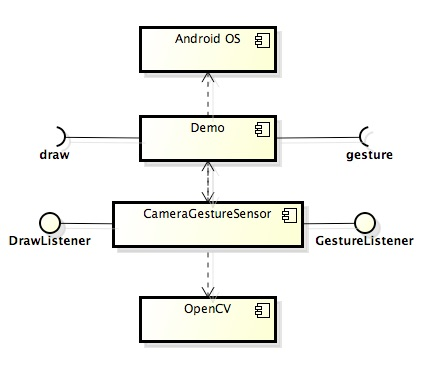
\includegraphics[width=0.5\textwidth ]{figure/demo}
    \caption{Demo组件图}
    \label{fg:demo}
\end{figure}
Demo的主类依赖于OpenCV,Android OS,与CameraGestureSensor为相互依赖关系。CameraGestureSensor需要Demo对OpenCV进行初始化,而Demo则需要CameraGestureSensor提供接口。Demo调用Android OS,实现前端渲染和相机控制。
\section{关键技术实现}
本节将具体叙述Demo中两个难点,即前端渲染函数和相机控制的具体实现。
\subsection{前端渲染}
\begin{itemize}
    \item 首先,我们在布局文件中放置一个SurfaceView用于手动绘制相机预览画面。
    \item 随后,将CameraGestureSensor传入的Mat利用BitMap转为一个位图
    \item 接着,利用当前缩放值scale,进行矩阵变换,绘制一副缩放后的位图
    \item 最后,锁定画布,将当前画面替换为缩放后的位图,解锁画布。一次绘制完成。
\end{itemize}
实际实现关键代码如下:
\begin{lstlisting}[language=JAVA]
Core.flip(currentFrame,currentFrame,1);
Bitmap bmp=processFrame(currentFrame);
Bitmap real;
if (bmp != null) {
    Canvas canvas = mView.getHolder().lockCanvas();
    if (canvas != null) {
        Matrix matrix = new Matrix();
        matrix.postRotate(90);
        matrix.postScale((float) 1.0 * canvas.getWidth() / bmp.getHeight(), (float) 1.0 * canvas.getHeight() / bmp.getWidth());
        real=Bitmap.createBitmap(bmp,0,0,bmp.getWidth(),bmp.getHeight(),matrix,true);
        if(scale!=1) {
            int x = (int) (canvas.getWidth() * (scale - 1) / 2.0);             int y = (int) (canvas.getHeight() * (scale - 1) / 2.0);
            matrix.reset();
            matrix.postScale(scale, scale);
            real = Bitmap.createBitmap(real, x, y, real.getWidth() - x, real.getHeight() - y, matrix, true);
        }
        if(is_taken==true){
            is_taken=false;
            takePicture(real);
        }
        canvas.drawBitmap(real, 0, 0, null);
        mView.getHolder().unlockCanvasAndPost(canvas);
        real.recycle();
    }
    bmp.recycle();
}  
\end{lstlisting}
需要注意的一点就是bmp最后一定要释放,否则则容易出现内存问题。
\subsection{相机控制}
相机控制无非有2种,一种是缩放,一种是拍照。

在前段渲染中,我们看见了在第三步时利用了一个缩放值进行绘制,实验中,我们就是利用此方法进行缩放的,也就是传统意义上的数字变焦。即利用一个scale记录变焦倍数,默认为1,恒大于1,小于5(因为大于5时已过于模糊,没有意义)。

而对于拍照,我们利用一个单独线程实现倒计时,当倒计时结束时我们直接将预览画面存至存储器中。需要注意的是在存储前要先判断存储文件夹是否存在,若不存在则需要自行新建。

\section{实验结果}

\subsection{Log记录}
图\ref{fg:1}为算法后台运行的log。可见,我们的间隔采集的理论速度应该是25FPS,但是由于软硬件性能因素实际只有16FPS,不过并不影响使用,仅为看起来略有卡顿。手势识别记录一切正常。
\begin{figure}[htb]
    \centering
    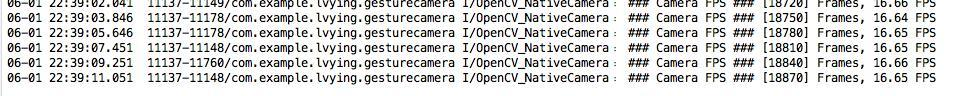
\includegraphics[width=0.5\textwidth ]{figure/opencvframe}%
    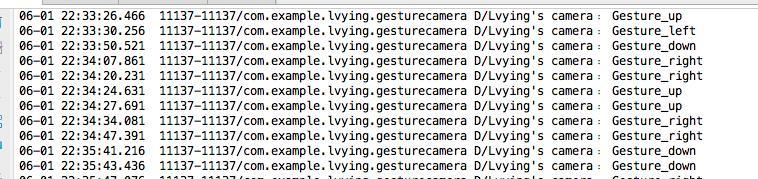
\includegraphics[width=0.5\textwidth ]{figure/gesture}
    \caption{log记录}
    \label{fg:1}
\end{figure}
\subsection{CPU与系统内存占用}
CPU与系统内存占用如图\ref{fg:2}所示。可见,本算法对内存及计算量的要求并不算高,并未占用太多系统资源,可以实际运用。
\begin{figure}[htb]
    \centering
    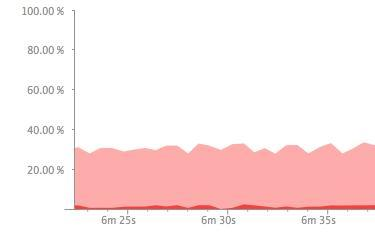
\includegraphics[width=0.5\textwidth ]{figure/cpu}%
    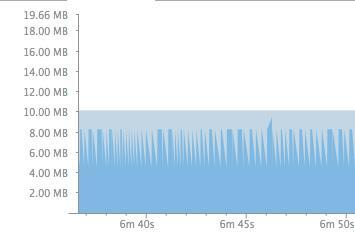
\includegraphics[width=0.5\textwidth ]{figure/memory}
    \caption{CPU与内存消耗占比图}
    \label{fg:2}
\end{figure}
\subsection{拍照实例}
当手势被识别后,进行对应功能处理。如果为左划则进入拍照功能,在屏幕右上角显示倒计时3秒,并在倒计时结束时拍照。如果是放大或缩小功能,由于前置摄像头无法实现物理变焦,故采用数字放大/缩小实现该功能。因为识别为动态过程,不方便截图展示,因此我们只截取了一个识别到左划手势并开始拍照倒计时的界面,和一个拍照完成的提示。如图\ref{fg:3}所示。
\begin{figure}[htb]
    \centering
    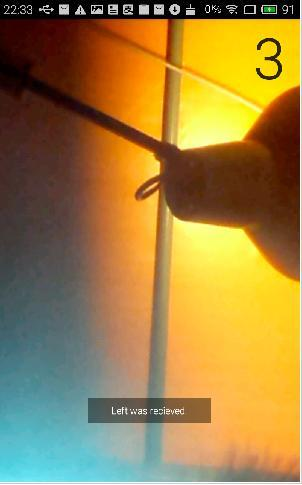
\includegraphics[width=0.3\textwidth ]{figure/recognize}%
    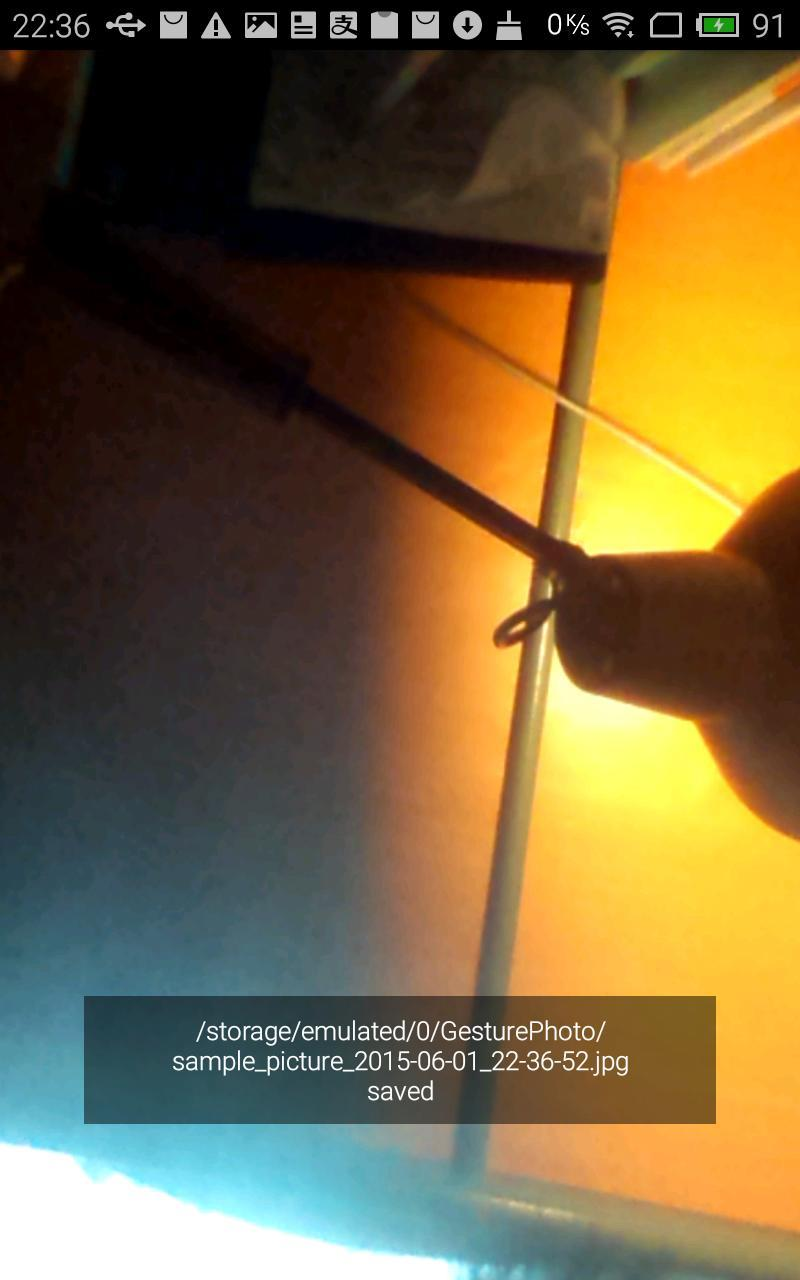
\includegraphics[width=0.3\textwidth ]{figure/capture}
    \caption{拍照展示}
    \label{fg:3}
\end{figure}

经过实验,本算法已具有一定的实际使用可行性,可以进行试验性使用。

\ifx\allfiles\undefined
%\bibliographystyle{unsrt}
\bibliography{main}
\end{document}
\fi